\section{View}
\label{chap:view_impl}
The view in this project is implemented based on the concept designed in \autoref{chap:view_design}
\subsection{MainActivity}
The user interface displays several functionalities to fulfill the requirements of the system described in \autoref{chap:requirements}. To promote separation of concerns, the user interface is implemented in several \texttt{Fragment}, improving the code readability and maintainability.  
\texttt{MainActivity} serves as the container that binds the fragments together. To host and display different fragments based on the user's navigation, \texttt{FragmentContainerView}\footnote{\url{FragmentContainerView} is a customized Layout designed specifically for Fragments. URL: \url{https://developer.android.com/reference/androidx/fragment/app/FragmentContainerView}} is used.
The navigation between the fragments is controlled by the Android Navigation\footnote{\url{Navigation} is a framework provided by the Android Jetpack library that simplifies the implementation of navigation in an Android app. URL: \url{https://developer.android.com/guide/navigation}}, which is configured in a XML file. 
\begin{lstlisting}[caption={Navigation graph snippet for HomeFragment (XML - nav\_Graph)}, language=XML]
<fragment
    android:id="@+id/homeFragment"
    android:name="com.ham.activitymonitorapp.fragments.HomeFragment"
    android:label="HomeFragment"
    tools:layout="@layout/home_fragment">
    <action
        android:id="@+id/action_homeFragment_to_userFragment"
        app:destination="@id/userFragment" />
    <action
        android:id="@+id/action_homeFragment_to_exercisesFragment"
        app:destination="@id/exercisesFragment" />
</fragment>
\end{lstlisting}

The \texttt{MainActivity} provides a bottom navigation tool for users to navigate between the fragments. It is implented using the BottomNavigationView\footnote{\url{BottomNavigationView} represents a standard bottom navigation bar for application. URL: \url{https://developer.android.com/reference/com/google/android/material/bottomnavigation/BottomNavigationView}}.
\begin{figure}[H]
    \centering
    
\includegraphics[width=0.75\textwidth]{images/bottom-navbar.png}
    \caption{Screenshot of the bottom navbar}
    \label{fig:bottom_navbar}
\end{figure}

Additionally, \texttt{MainActivity} manages permission requests to ensure the necessary permissions are granted for the app's functionality. Specifically, it requests the \texttt{ACCESS\_COARSE\_LOCATION} permission.

\subsection{HomeFragment}
The implementation of \texttt{HomeFragment} includes several feature to fulfill the requirements of the system. 
Firstly, it provides a switch to control the connection to the heart rate sensor. This feature is disabled when there is no active user.

Moreover, the fragment displays the user's current heart rate (bpm) by observing the \texttt{currentHrBpm} LiveData from the \texttt{HrViewModel}. This ensures that the displayed heart rate is always up-to-date.
Additionally, the \texttt{HomeFragment} shows the user's current activity intensity level by observing the \texttt{currentActivity} LiveData also provided by the \texttt{HrViewModel}. 
\begin{lstlisting}[caption={Observers for currentActivity and currentHrBpm (HomeFragment)}]
    private fun observeHrData() {
        hrViewModel.currentHrBpm.observe(viewLifecycleOwner) { newHrData ->
            binding.heartRate.text = newHrData.toString()
        }
    }
    private fun observeActivity() {
        hrViewModel.currentActivity.observe(viewLifecycleOwner) { newActivity ->
            binding.activityMonitor.text = "Activity: $newActivity"
        }
    }
\end{lstlisting}

Furthermore, the fragment features an interactive graph that visualizes the user's heart rate data over time. 
The graph is controlled by another component called \texttt{GraphService} using the MPAndroidChart library, specifically the \texttt{LineChart} class.
The \texttt{GraphService} subscribes to the \texttt{HrEventBus}, which broadcasts heart rate data events. 
Whenever a heart rate data event is received, the \texttt{GraphService} updates the data set associated with the graph. 
This ensures that the graph is continuously updated with the latest heart rate data.
Additionally, the \texttt{GraphService} also reacts to changes in the active user. 
When the active user is changed, the \texttt{GraphService} generates a new graph based on the heart rate data of the new active user. 

Lastly, the \texttt{HomeFragment} observes the current active user and dynamically updates the user interface to display the current heart rate, activity level, and the graph.
\begin{figure}[H]
    \centering
    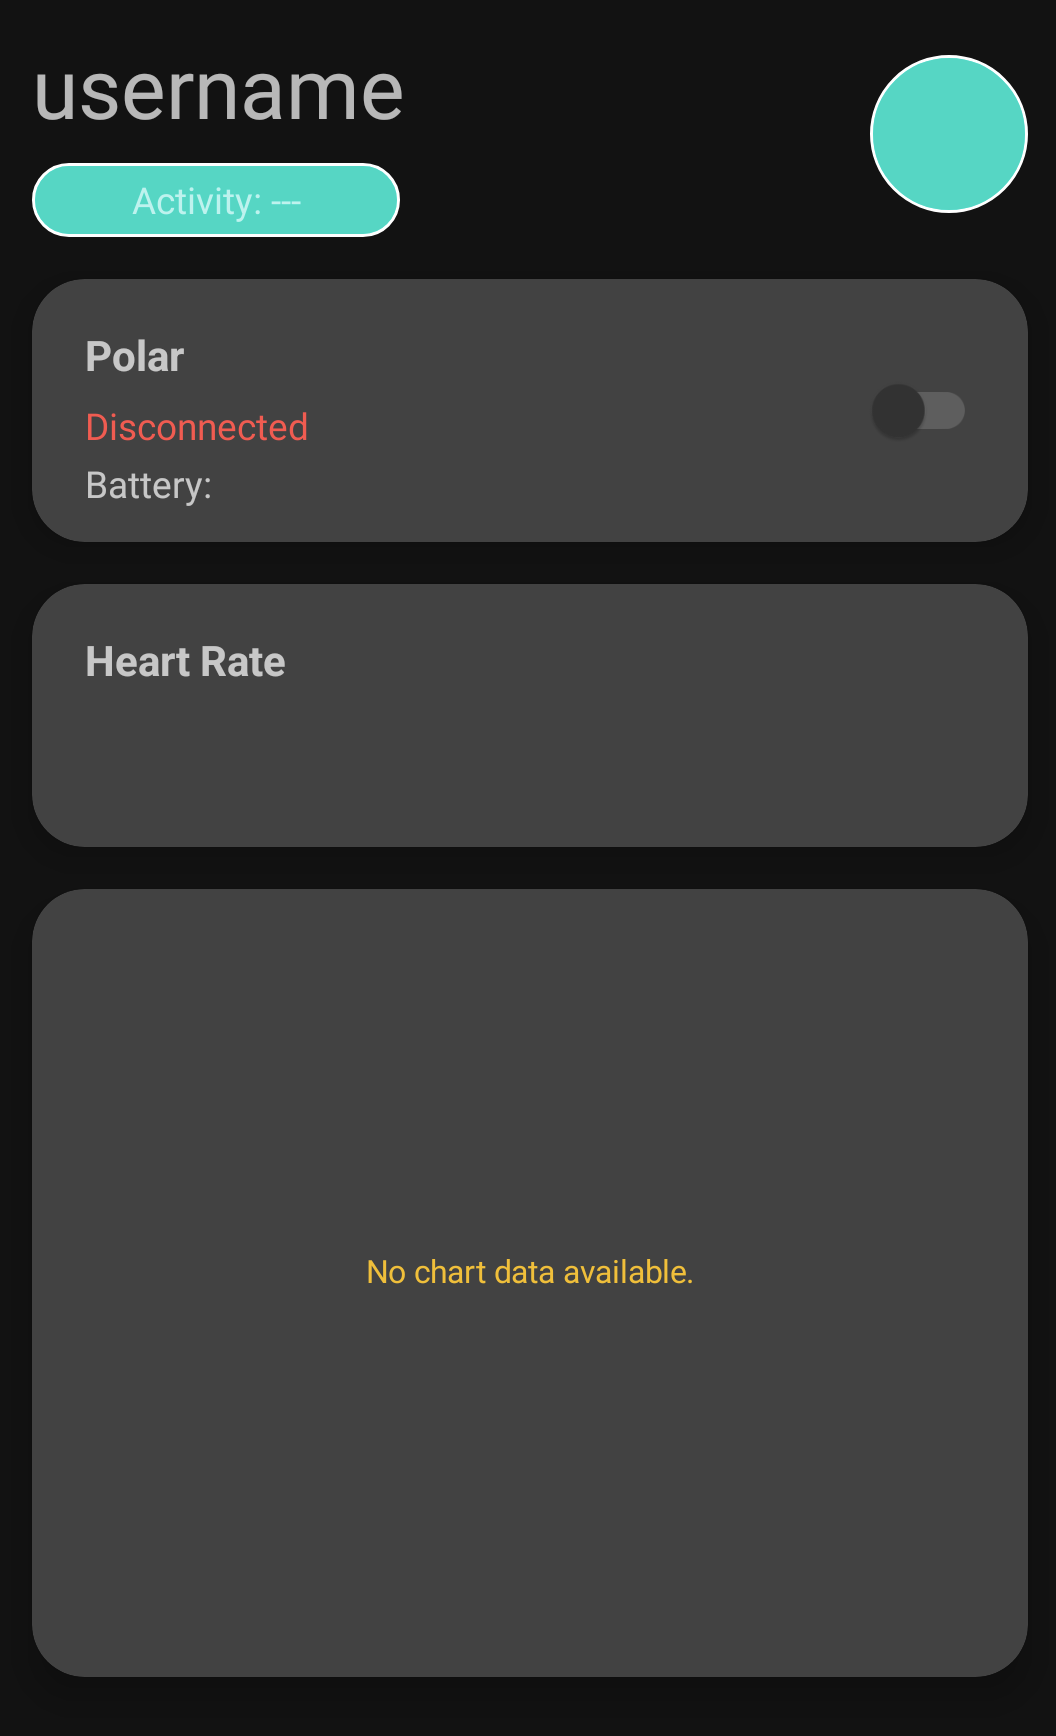
\includegraphics[width=0.4\textwidth]{images/homefragment-screenshot.png}
    \caption{Screenshot of HomeFragment}
    \label{fig:homefragment_screenshot}
\end{figure}

\subsection{ExerciseFragment}
The \texttt{ExerciseFragment} shows an overview of an ongoing exercise. It uses \texttt{DataBinding} to display the exercise details and observing the \texttt{currentExercise} LiveData from the \texttt{ExerciseViewModel}. 
\begin{lstlisting}[caption={Observer for currentExercise (HomeFragment)}]
private fun observeAndUpdateExercise() {
    exerciseViewModel.currentExercise.observe(viewLifecycleOwner) { newExercise ->
        binding.includeExerciseStart.exercise = newExercise
    }
}
\end{lstlisting}

The \texttt{ExerciseFragment} also offers buttons to start and stop an exercise session.
Once the user presses the button to start an exercise session and the process is successfully started, the start button will be automatically disabled to prevent multiple start requests. Similarly, when the stop button is pressed, the stop button will also be disabled to avoid any unintended interruptions. 
This approach ensures that the exercise can be performed without any conflicting or overlapping commands.
To ensure accurate data, the \texttt{ExerciseFragment} observes the current active user and adjusts the exercise information accordingly.

Additionally, a separate fragment called \texttt{ExerciseListFragment} is created inside the \texttt{ExerciseFragment} to display a list of completed exercises. The \texttt{ExerciseFragment} observes \texttt{currentExerciseList} live data from the \texttt{ExerciseViewModel} to receive updates. 
\texttt{RecyclerView}\footnote{\url{RecyclerView} is widget used for displaying sets of data efficiently. URL: \url{https://developer.android.com/reference/androidx/recyclerview/widget/RecyclerView}} widget is used to dynamically display the \texttt{currentExerciseList}. 
\begin{lstlisting}[caption={Observer for currentExercise (HomeFragment)}]
private fun observeExerciseList() {
    exerciseViewModel.currentExercisesList.observe(viewLifecycleOwner) { newExercisesList ->
        initRecyclerView(newExercisesList)
    }
}
\end{lstlisting}
\begin{figure}[H]
    \centering
    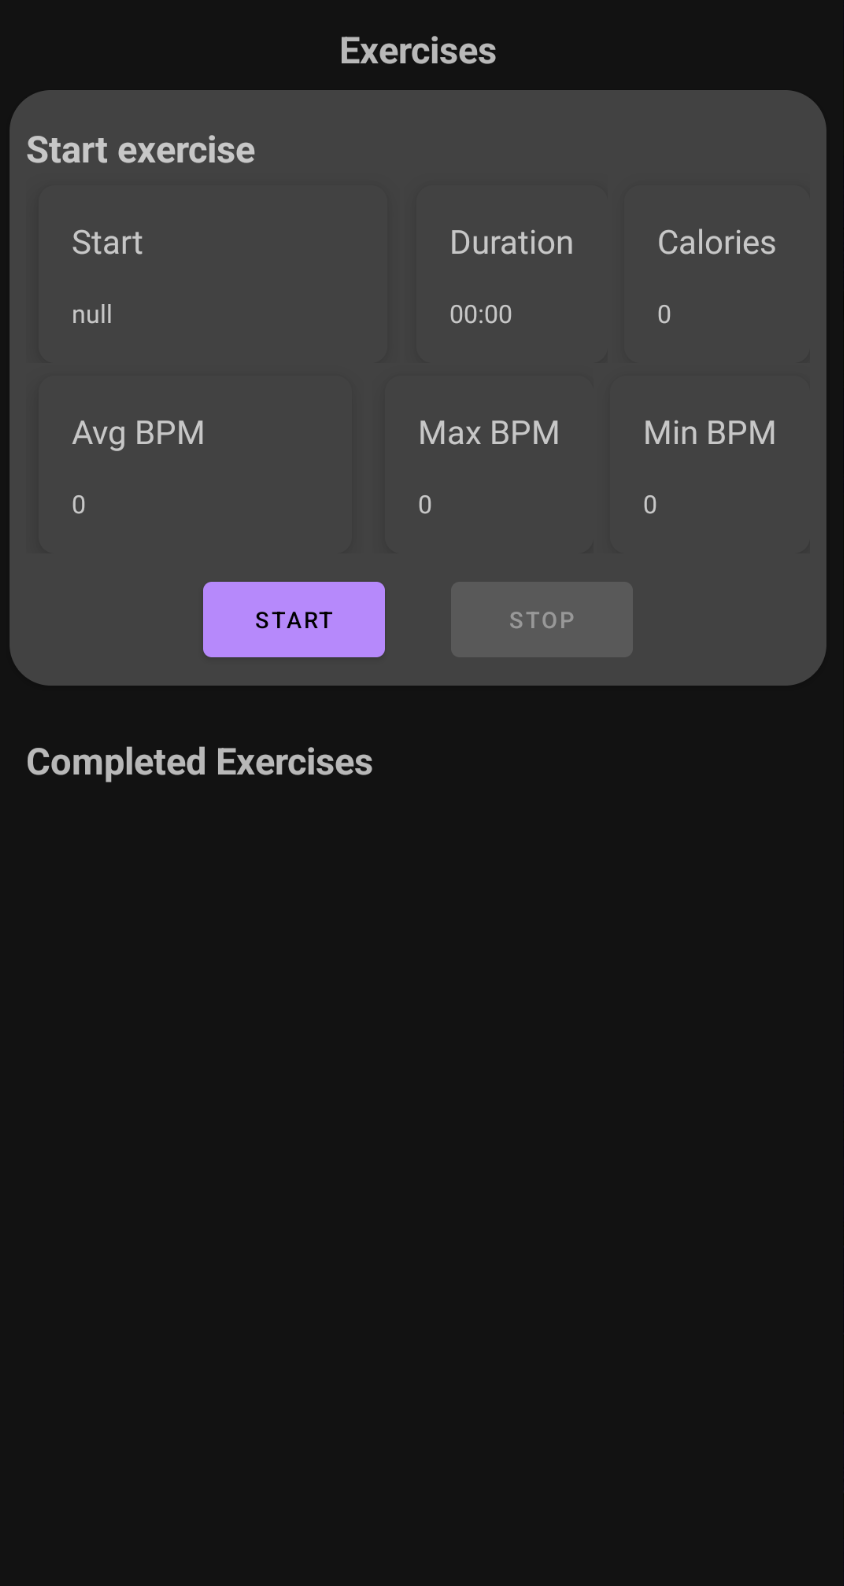
\includegraphics[width=0.5\textwidth]{images/exercisefragment-screenshot.png}
    \caption{Screenshot of ExerciseFragment}
    \label{fig:userfragment_screenshot}
\end{figure}

\subsection{UserFragment}
The \texttt{UserFragment} is responsible for displaying the details of the current active user. 
To achieve this functionality, it observes the \texttt{currentUser} LiveData from the \texttt{UserViewModel} and bind it using \texttt{DataBinding}. 
\begin{lstlisting}[caption={Observer for currentUser (UserFragment)}]
private fun observeActiveUser() {
    userViewModel.activeUser.observe(viewLifecycleOwner) { user ->
        binding.activeUser = user
    }
}
\end{lstlisting}
The user information is displayed in text fields and a calendar is available to support adding or editing the date of birth. 
Additionally, \texttt{UserFragment} provides three buttons for deleting, adding, and updating user data.
\begin{figure}[H]
    \centering
    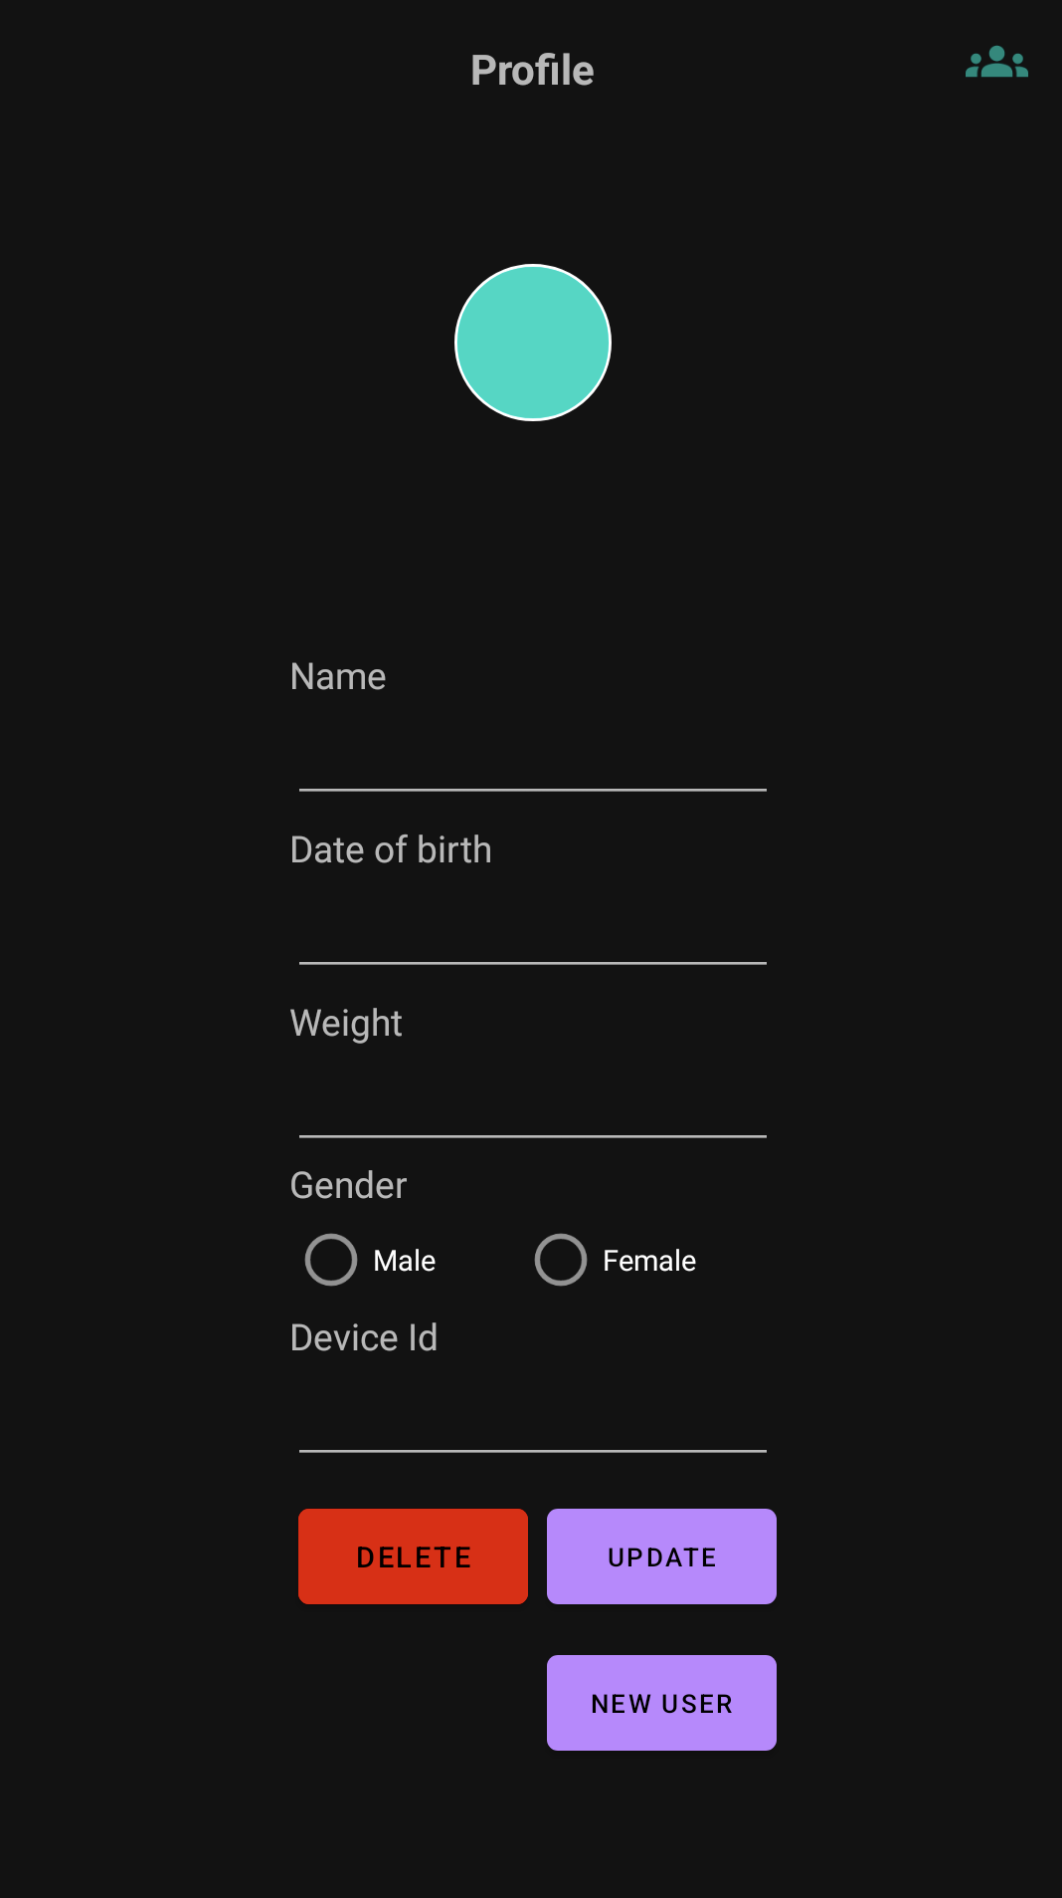
\includegraphics[width=0.5\textwidth]{images/userfragment-screenshot.png}
    \caption{Screenshot of UserFragment}
    \label{fig:userfragment_screenshot}
\end{figure}

Furthermore, a separate \texttt{UserListFragment} is implemented to display a list of all users in the system. 
Similar to the \texttt{ExerciseListFragment}, it uses a \texttt{RecyclerView} to display a list of users. 
Each user in the list is clickable, allowing the user to change the active user by selecting a different user from the list.


